\documentclass[12pt]{article}    
\usepackage{ucs} 
\usepackage[utf8x]{inputenc}
\usepackage[russian]{babel}  
\title{Лабораторная работа №6\\Определение коэффициента трения скольжения}
\author{Хафизов Фанис}
\usepackage[pdftex]{graphicx}



\begin{document}
	\begin{figure}
		\centering
		
\includegraphics[width=0.3\linewidth]{logo}
	\end{figure}
	\maketitle
	\newpage
	\section{Цель работы:}
	Изучить закон сухого трения и ознакомиться с методами определения коэффициента трения скольжения.
	\section{Схема установки:}
	\begin{figure}[h]
		\centering
		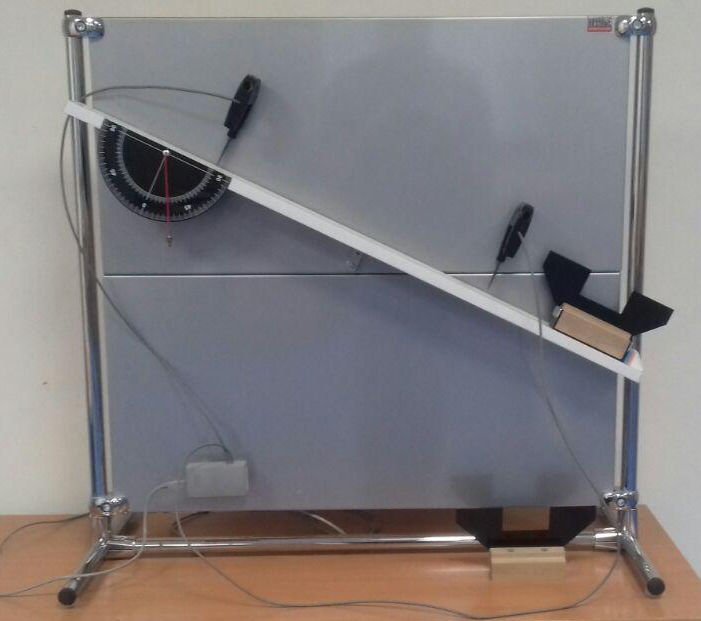
\includegraphics[width=0.7\linewidth]{image1}
		\caption{Схема установки}
		\label{fig:image1}
	\end{figure}
	Лабораторный стенд (рис. 1) включает наклонную направляющую скамью
	с прикрепленной к ней измерительной линейкой, движущееся тело (2 шт.),
	оптоэлектрические датчики (2 шт.) с модулем сбора сигналов, а также
	транспортир для измерения угла наклона направляющей скамьи. К приборам
	и принадлежностям относятся также компьютер с необходимым программным
	обеспечением.
	\section{Порядок действий}
	1)Соберём экспериментальную установку, выставив угол наклона $\alpha=30^{\circ}$ и установив датчики на достаточном расстоянии друг от друга.
	\newline
	2)С помощью соединительного кабеля подключим к компьютеру модуль
	сбора сигналов, к которому присоединены датчики. Затем откроем программу для получения результатов на компьютере.
	\newline
	3)Установим брусок в верхней точке линейки. Запустим измерения и отпустим брусок. После остановки бруска закончим запись. Обработаем
	данные по прохождению через датчики и найдем ускорение в каждом случае.
	\section{Таблицы данных и графики}
		\begin{table}[h]
		\caption{Входные данные}
		\begin{tabular}{|c|c|c|c|c|c|c|c|c|c|c|}
			\hline
			№&$\alpha,$&$l,$&$x_1,$&$x_1+l,$&$x_1+2l,$&$x_1+3l,$&$x_2,$&$x_2+l,$&$x_2+2l,$&$x_2+3l,$\\
			п/п&$^{\circ}$&мм&мм&мм&мм&мм&мм&мм&мм&мм\\
			\hline
			1&30&70&250&320&390&460&650&720&790&860\\
			1&30&70&200&270&340&410&600&670&740&810\\
			1&30&70&200&270&340&410&550&620&690&760\\
			1&30&70&200&270&340&410&500&570&640&710\\
			1&30&70&250&320&390&460&600&670&740&810\\
			\hline
			2&30&70&250&320&390&460&650&720&790&860\\
			2&30&70&250&320&390&460&600&670&740&810\\
			2&30&70&250&320&390&460&550&620&690&760\\
			2&30&70&250&320&390&460&500&570&640&710\\
			2&30&70&200&270&340&410&600&670&740&810\\
			\hline
		\end{tabular}
	\end{table}
	\begin{table}[h!]
		\caption{Значения ускорений и коэффициента трения}
		\begin{tabular}{|c|c|c|c|c|c|c|c|c|}
			\hline
			№&$a_1,$&$a_2,$&$a_3,$&$a_4,$&$a_5,$&$\overline{a},$&$\mu$&$\Delta\mu$\\
			п/п&м/с$^2$&м/с$^2$&м/с$^2$&м/с$^2$&м/с$^2$&м/с$^2$&&\\
			\hline
			1&1,520&1,538&1,788&1,520&1,506&1,574&0,392&0,025\\
			2&1,236&1,482&1,214&1,182&1,224&1,268&0,428&0,026\\
			\hline
		\end{tabular}
	\end{table}
	\begin{figure}[h!]
		\centering
		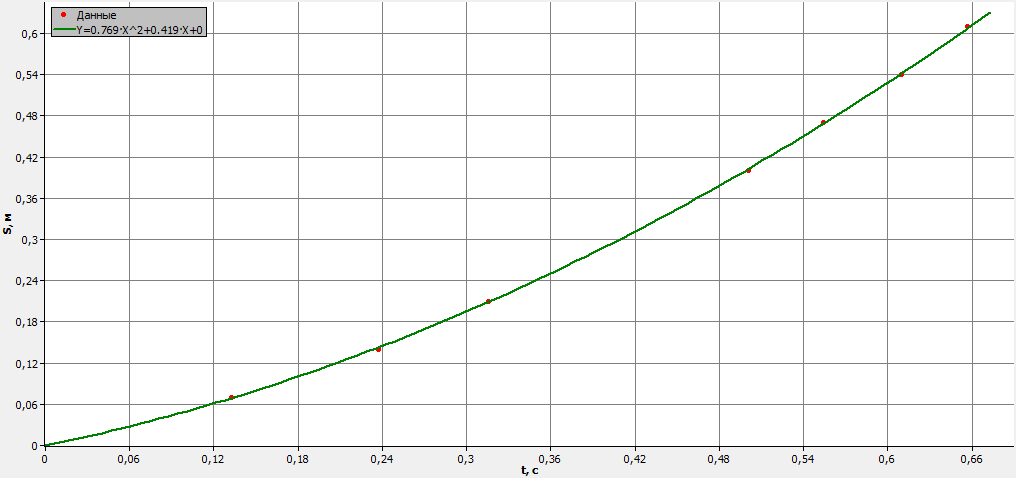
\includegraphics[width=1\linewidth]{graph1.png}
		\caption{График зависимости S(t) для первого бруска}
		\label{fig:graph1}
	\end{figure}
	\begin{figure}[h!]
		\centering
		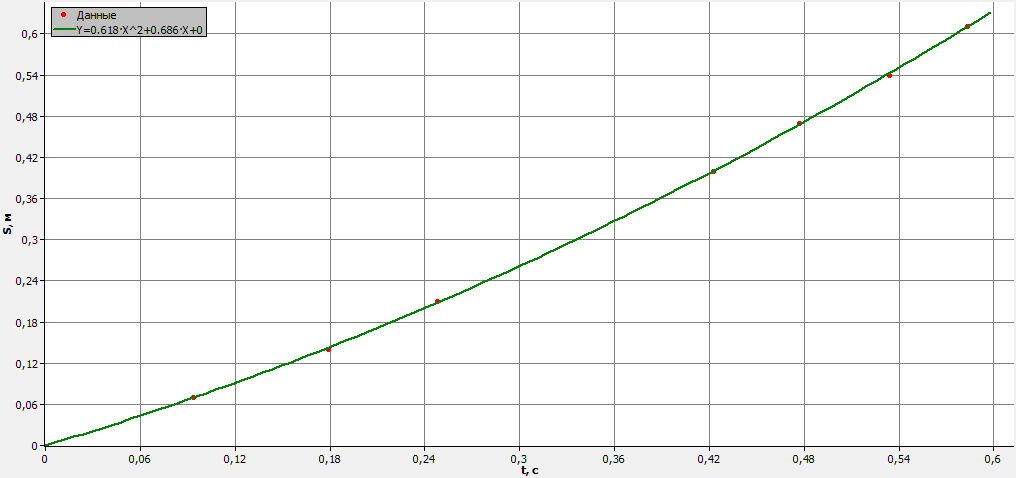
\includegraphics[width=1\linewidth]{graph2.png}
		\caption{График зависимости S(t) для второго бруска}
		\label{fig:graph1}
	\end{figure}
	\section{Расчеты}
	$\overline{a}=\frac{\sum\limits_{i=1}^{5} a_i}{5}$
	\newline
	$\overline{\mu}=tg\alpha-\frac{\overline{a}}{gcos\alpha}$
	\newline
	$\overline{\mu}_1=tg30^{\circ}-\frac{1,574}{gcos30^{\circ}}=\frac{1}{\sqrt{3}}-\frac{1,574}{9,8\cdot\frac{\sqrt{3}}{2}}=0,392$
	\newline
	$\overline{\mu}_2=tg30^{\circ}-\frac{1,268}{gcos30^{\circ}}=\frac{1}{\sqrt{3}}-\frac{1,268}{9,8\cdot\frac{\sqrt{3}}{2}}=0,428$
	\newline
	Расчет погрешностей:\\
	$\Delta a=2\sqrt{\frac{\sum \limits_{i=1}^{5} (a_i-\overline{a})^2}{5}}$\\
	$\Delta a_1=0,215$м/с$^2$\\
	$\Delta a_2=0,217$м/с$^2$\\
	$\Delta \mu=\frac{\Delta a}{gcos\alpha}$\\
	$\Delta \mu_1=\frac{\Delta a_1}{gcos\alpha}=\frac{0,215}{9,8\cdot\frac{\sqrt{3}}{2}}=0,025$\\
	$\Delta \mu_2=\frac{\Delta a_2}{gcos\alpha}=\frac{0,217}{9,8\cdot\frac{\sqrt{3}}{2}}=0,026$\\
	$\varepsilon_\mu=\frac{\Delta \mu}{\overline{\mu}}$\\
	$\varepsilon_{\mu1}=\frac{\Delta {\mu_1}}{\overline{\mu}_1}=\frac{0,025}{0,392}=6\%$\\
	$\varepsilon_{\mu2}=\frac{\Delta {\mu_2}}{\overline{\mu}2}=\frac{0,026}{0,428}=6\%$\\
	\section{Результаты}
	$\mu=\overline{\mu}\pm \Delta \mu$\\
	$\mu_1=\overline{\mu}_1\pm \Delta \mu_1=0,392\pm0,025$\\
	$\mu_2=\overline{\mu}_2\pm \Delta \mu_2=0,428\pm0,026$\\
	\section{Вывод}
	Мы получили достаточно ожидаемый результат. Необычно лишь то, что коэффициент трения у обоих брусков получился почти одинаковый. Относительная погрешность в обоих случаях 6\%. Основная составляющая погрешности -- случайная погрешность измерений. Для улучшения точности результата можно было бы увеличить длину линейки или использовать больше датчиков.
	\end{document}